\documentclass[tikz,border=6pt]{standalone}
\usepackage[T1]{fontenc}
\usepackage{mathptmx}\usepackage{courier}
\usetikzlibrary{positioning,arrows.meta,fit,backgrounds,calc}
\definecolor{stA}{HTML}{E6EBF5}\definecolor{stB}{HTML}{E2F7F6}\definecolor{stC}{HTML}{F8F1E6}
\definecolor{gvArb}{HTML}{4A0C6E}\definecolor{gvBrick}{HTML}{BA6F4C}\definecolor{edge}{HTML}{3A3A3A}\definecolor{acc}{HTML}{0032A0}
\tikzset{
  box/.style={draw=edge, line width=0.6pt, rounded corners=2pt, fill=white, align=center,
              font=\small, minimum height=11mm, text width=33mm, inner sep=3pt},
  data/.style={box, fill=gray!8},
  db/.style={draw=edge, line width=0.6pt, fill=white, align=center, font=\small,
             shape=rectangle, text width=26mm, minimum height=13mm},
  rule/.style={box, text width=30mm, minimum height=9mm, font=\footnotesize},
  res/.style={box, line width=0.9pt, draw=acc, text width=33mm},
  arr/.style={-{Stealth[length=2.2mm]}, line width=0.7pt, draw=edge},
  stage/.style={rounded corners=4pt, inner sep=7pt},
  stitle/.style={font=\bfseries\small, anchor=north west, inner sep=2pt},
  bdg/.style={circle, font=\bfseries\tiny, text=white, inner sep=0pt, minimum size=4.2mm},
  bP/.style={bdg, fill=gray!70},
  bM/.style={bdg, fill=gvArb},
  bO/.style={bdg, fill=gvBrick},
  num/.style={circle, fill=acc, text=white, font=\bfseries\scriptsize, inner sep=1.2pt, minimum size=4mm},
}
\begin{document}
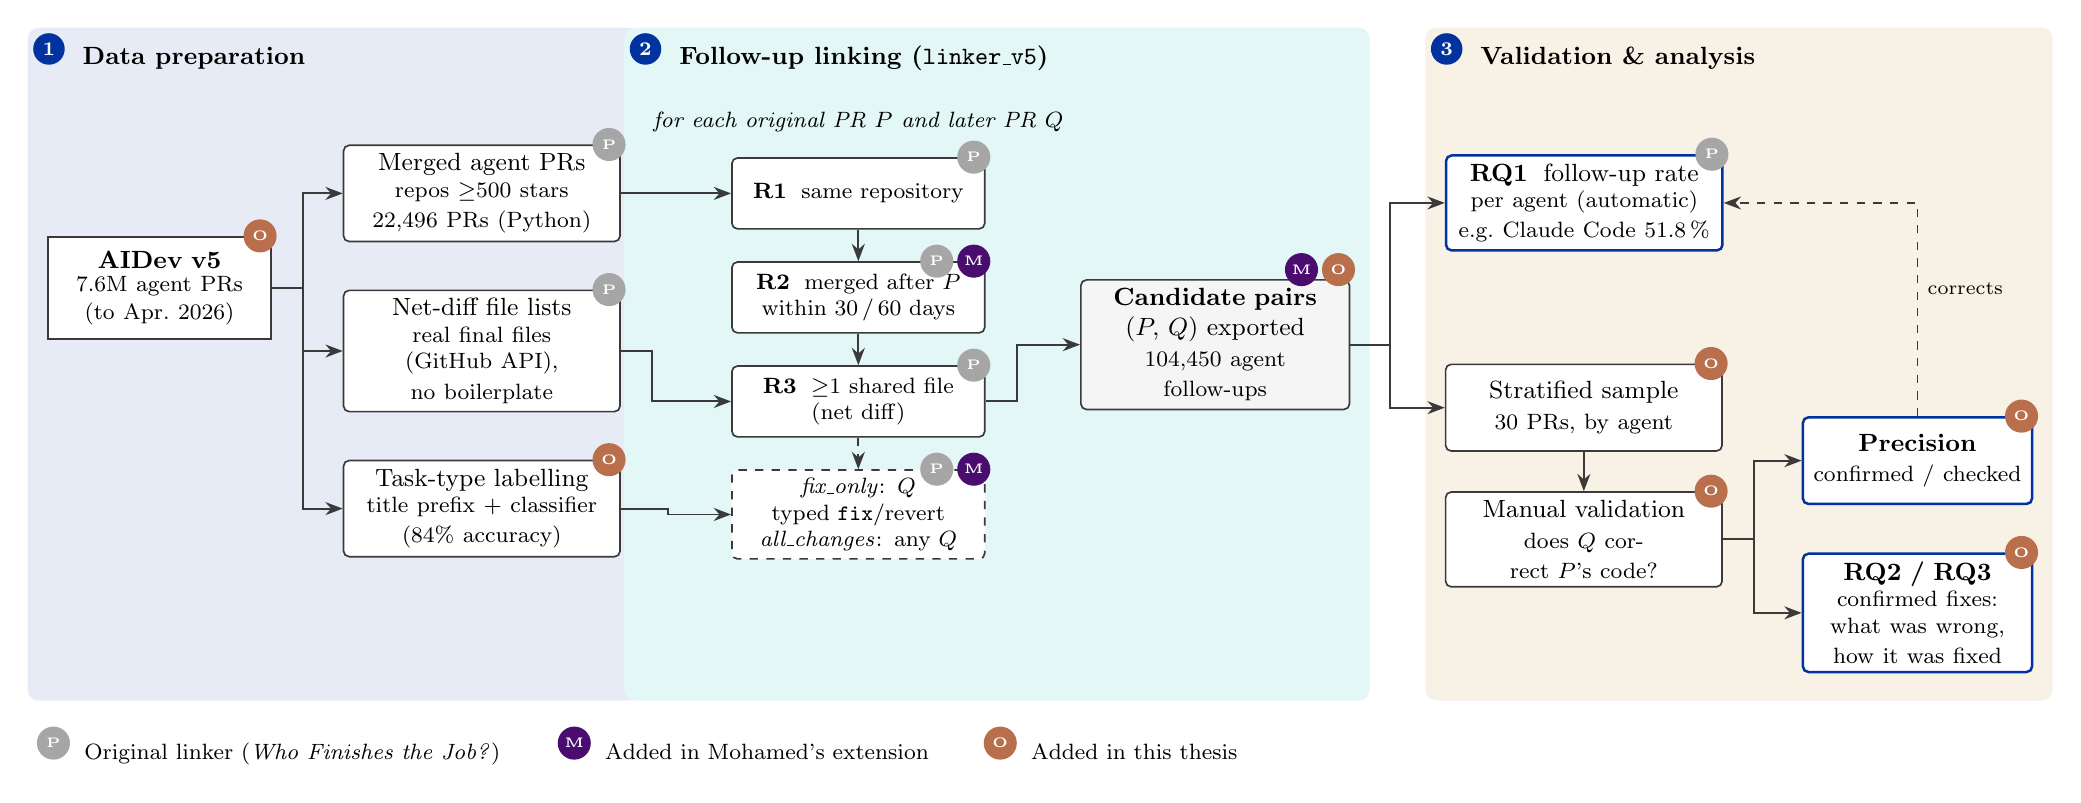
\begin{tikzpicture}[node distance=6mm and 9mm]

% ---------------- Stage A: data preparation ----------------
\node[db] (aidev) {\textbf{AIDev v5}\\[-1pt]\footnotesize 7.6M agent PRs\\[-1pt]\footnotesize (to Apr.\ 2026)};
\node[box, right=of aidev, yshift=12mm] (pop) {Merged agent PRs\\ \footnotesize repos $\geq$500 stars\\ \footnotesize 22{,}496 PRs (Python)};
\node[box, below=of pop] (files) {Net-diff file lists\\ \footnotesize real final files (GitHub API),\\ \footnotesize no boilerplate};
\node[box, below=of files] (type) {Task-type labelling\\ \footnotesize title prefix $+$ classifier\\ \footnotesize (84\% accuracy)};
\draw[arr] (aidev.east) -- ++(4mm,0) |- (pop.west);
\draw[arr] (aidev.east) -- ++(4mm,0) |- (type.west);
\draw[arr] (aidev.east) -- ++(4mm,0) |- (files.west);

% ---------------- Stage B: follow-up linking ----------------
\node[rule, right=14mm of pop] (r1) {\textbf{R1}\; same repository};
\node[rule, below=4mm of r1] (r2) {\textbf{R2}\; merged after $P$\\ within 30\,/\,60 days};
\node[rule, below=4mm of r2] (r3) {\textbf{R3}\; $\geq$1 shared file\\ \footnotesize (net diff)};
\node[rule, below=4mm of r3, dashed] (r4) {\footnotesize\textit{fix\_only}: $Q$ typed \texttt{fix}/revert\\ \textit{all\_changes}: any $Q$};
\draw[arr] (r1) -- (r2); \draw[arr] (r2) -- (r3); \draw[arr, dashed] (r3) -- (r4);
\node[font=\footnotesize\itshape, above=2mm of r1] (pq) {for each original PR $P$ and later PR $Q$};

\node[data, right=12mm of r2, yshift=-6mm, text width=32mm] (pairs) {\textbf{Candidate pairs}\\ $(P,\,Q)$ exported\\ \footnotesize 104{,}450 agent follow-ups};
\draw[arr] (r3.east) -- ++(4mm,0) |- (pairs.west);

% ---------------- Stage C: validation & analysis ----------------
\node[res, right=12mm of pairs, yshift=18mm] (rate) {\textbf{RQ1}\; follow-up rate\\ \footnotesize per agent (automatic)\\ \footnotesize e.g.\ Claude Code 51.8\,\%};
\node[box, right=12mm of pairs, yshift=-8mm] (sample) {Stratified sample\\ \footnotesize 30 PRs, by agent};
\node[box, below=5mm of sample] (manual) {Manual validation\\ \footnotesize does $Q$ correct $P$'s code?};
\node[res, right=10mm of manual, yshift=10mm, text width=27mm] (prec) {\textbf{Precision}\\ \footnotesize confirmed / checked};
\node[res, below=of prec, text width=27mm] (q23) {\textbf{RQ2 / RQ3}\\ \footnotesize confirmed fixes:\\ what was wrong,\\ how it was fixed};
\draw[arr] (pairs.east) -- ++(5mm,0) |- (rate.west);
\draw[arr] (pairs.east) -- ++(5mm,0) |- (sample.west);
\draw[arr] (sample) -- (manual);
\draw[arr] (manual.east) -- ++(4mm,0) |- (prec.west);
\draw[arr] (manual.east) -- ++(4mm,0) |- (q23.west);
\draw[arr, dashed] (prec.north) |- node[pos=0.3,right,font=\scriptsize]{corrects} (rate.east);

% connections between stages
\draw[arr] (pop.east) -- (r1.west);
\draw[arr] (type.east) -- ++(6mm,0) |- (r4.west);
\draw[arr] (files.east) -- ++(4mm,0) |- (r3.west);

% ---------------- stage backgrounds ----------------
\begin{scope}[on background layer]
  \coordinate (T) at ($(pq.north)+(0,7mm)$);
  \coordinate (B) at ($(q23.south)+(0,-1mm)$);
  \node[stage, fill=stA, fit=(aidev)(pop)(type)(T -| pop)(B -| pop)] (SA) {};
  \node[stage, fill=stB, fit=(pq)(r1)(r4)(pairs)(T -| r1)(B -| r1)] (SB) {};
  \node[stage, fill=stC, fit=(rate)(sample)(manual)(prec)(q23)(T -| rate)(B -| rate)] (SC) {};
\end{scope}
\node[stitle] at (SA.north west) {\tikz\node[num]{1};\; Data preparation};
\node[stitle] at (SB.north west) {\tikz\node[num]{2};\; Follow-up linking (\texttt{linker\_v5})};
\node[stitle] at (SC.north west) {\tikz\node[num]{3};\; Validation \& analysis};

% ---------------- origin badges: P = paper, M = Mohamed, O = ours ----------------
\newcommand{\tag}[3][]{\node[#2, anchor=center] at ($(#3.north east)+(-1.2mm,0)$) {#1};}
\node[bO] at ($(aidev.north east)+(-1.5mm,0)$) {O};
\node[bP] at ($(pop.north east)+(-1.5mm,0)$) {P};
\node[bP] at ($(files.north east)+(-1.5mm,0)$) {P};
\node[bO] at ($(type.north east)+(-1.5mm,0)$) {O};
\node[bP] at ($(r1.north east)+(-1.5mm,0)$) {P};
\node[bP] at ($(r2.north east)+(-6.2mm,0)$) {P};\node[bM] at ($(r2.north east)+(-1.5mm,0)$) {M};
\node[bP] at ($(r3.north east)+(-1.5mm,0)$) {P};
\node[bP] at ($(r4.north east)+(-6.2mm,0)$) {P};\node[bM] at ($(r4.north east)+(-1.5mm,0)$) {M};
\node[bM] at ($(pairs.north east)+(-6.2mm,1.2mm)$) {M};\node[bO] at ($(pairs.north east)+(-1.5mm,1.2mm)$) {O};
\node[bP] at ($(rate.north east)+(-1.5mm,0)$) {P};
\node[bO] at ($(sample.north east)+(-1.5mm,0)$) {O};
\node[bO] at ($(manual.north east)+(-1.5mm,0)$) {O};
\node[bO] at ($(prec.north east)+(-1.5mm,0)$) {O};
\node[bO] at ($(q23.north east)+(-1.5mm,0)$) {O};
% legend
\node[font=\footnotesize, anchor=north west] at ($(SA.south west)+(0,-2mm)$) {%
  \tikz\node[bP]{P};\; Original linker (\textit{Who Finishes the Job?}) \qquad
  \tikz\node[bM]{M};\; Added in Mohamed's extension \qquad
  \tikz\node[bO]{O};\; Added in this thesis};
\end{tikzpicture}
\end{document}
